\chapter{图论 - 树}

\begin{figure}[ht]
  \centering
  \includegraphics[width=1\textwidth]{asset/茶桁的 AI 秘籍_Math_26.png}
\end{figure}

\newpage

这一节课是我们 AI 秘籍整个数学篇的最后一节课. 同样的, 这节课的概念还是比较重要的. 我们要来了解一下「树」. 

\section{树}

树其实是图的一种, 首先呢它是一个连通图, 是一个不含圈的连通图. 

什么叫连通图呢?连通图其实很简单, 就是任意两个顶点, 都有一条路径能使它们相连. 

\begin{figure}[ht]
  \centering
  \begin{minipage}[t]{0.2\textwidth}
    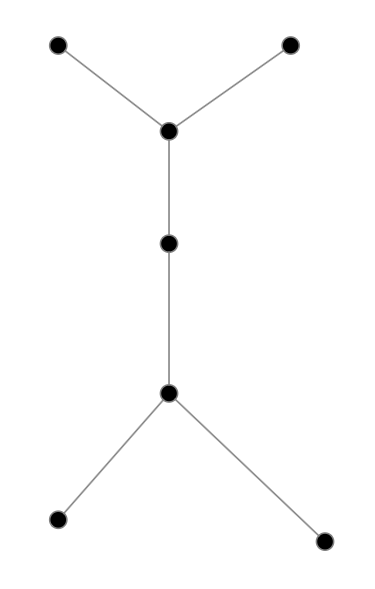
\includegraphics[width=\textwidth]{asset/20230924092520.png}
    \caption{}
    \label{fig:img27_1}
  \end{minipage}%
  \hspace{1em}
  \begin{minipage}[t]{0.3\textwidth}
    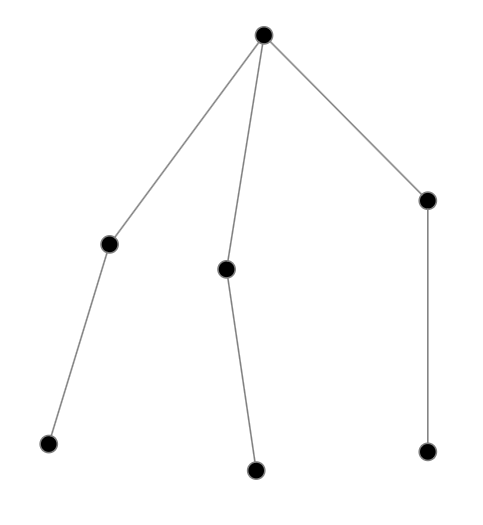
\includegraphics[width=\textwidth]{asset/20230924092635.png}
    \caption{}
    \label{fig:img27_2}
  \end{minipage}%
\end{figure}

比如图 \ref{fig:img27_1} 中左下角的点和右上角的点, 它们俩虽然不直接相连, 但是它们可以通过路径可以相连. 所以这两个点就具有这个连通性. 

如果一个图里面任意两个点都具有连通性的话, 那这个图呢就叫做连通图. 连通图就是从任意一个点出发都能去到剩下的所有点, 都有这样的路径. 这个就很像我们地铁换乘一样, 即便我从 a 地到 b 地不一定有直达的地铁, 但是我可以在中转站换一下地铁可以到达. 

连通图之外它还有一个限定, 叫做「不含圈的」. 比如我们在上一节课的那张图: 

\begin{figure}[ht]
  \centering
  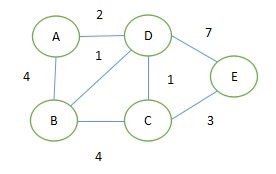
\includegraphics[width=0.4\textwidth]{asset/20230924051221.jpg}
  \caption{}
  \label{fig:img27_3}
\end{figure}

在图\ref{fig:img27_3}里面, 形成了闭合的一个圈. 我如果沿着 ADBA 的路径, 就能从起点再回到起点. 树是不含圈的连通图, 所以在图\ref{fig:img27_4}中的两个图, 我们都把它称为树: 

\begin{figure}[ht]
  \centering
  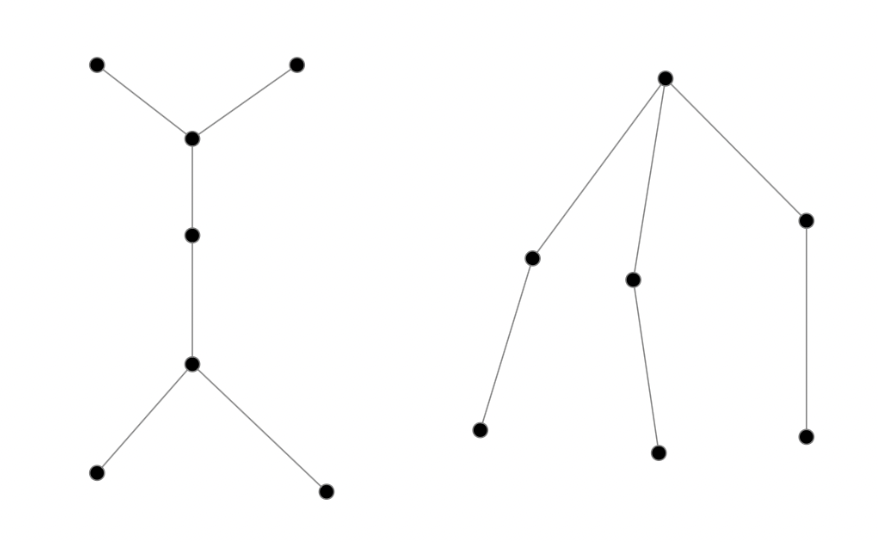
\includegraphics[width=0.5\textwidth]{asset/20230924093316.png}
  \caption{}
  \label{fig:img27_4}
\end{figure}

大家可以去验证一下, 首先它不含圈很明显;其次它任意两个点之间都是具有连通性的, 从任意一个点出发都可以去到其他任意一个点. 这就是树的一个定义. 

\section{生成树}

接下来, 我们再来看一下生成树又是怎么一回事. 

生成树是包含连通图里面的所有顶点的树, 而且任意两个连通的顶点之间有且仅有一条边, 它就不会有重边的这种情况出现. 然后还有一个性质就是它顶点数减去边数是 1. 

这个很像我们把一个法式长棍给它切三刀, 三刀把这个面包切成了四份. 在这里每一刀就相当于给他加了一条边, 然后切的那一小块就相当于顶点. 比如说我们在平面里面要连接三个点, 需要两个线段, 都是点数减 1. 

生成树就是这么一个含义, 首先包含了这个图里面的所有顶点, 之后是任意的两个连通的顶点之间是不会有重复路径的. 

\begin{figure}[ht]
  \centering
  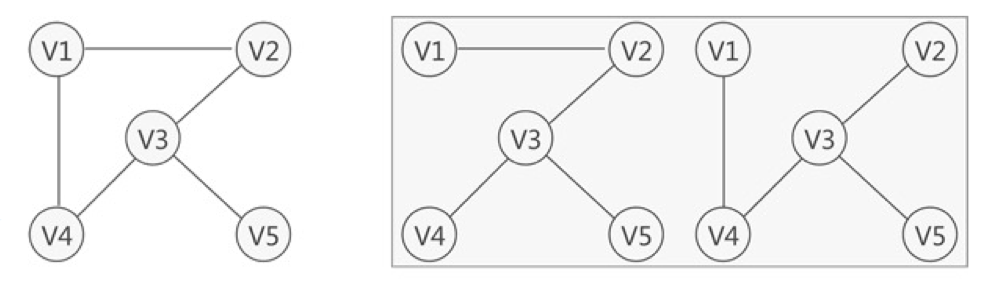
\includegraphics[width=0.8\textwidth]{asset/9560c897-3d1c-4169-9c28-681e0ccc1251.png}
  \caption{}
  \label{fig:img27_5}
\end{figure}

我们来看一下图 \ref{fig:img27_5} 中的左图. 对于这个图而言, 它不是一个树, 因为我们说过树是不能有圈的. 很明显这种结构不是一个树. 但是我们又想涵盖这个图里所有的顶点. 既然想涵盖这里面所有的顶点怎么办呢?就去找生成树, 要找到生成树就要按照规则去找, 所以我们可以有按照不同的去边的方法找到不同的生成树. 

右边的框里这两种生成树呢其实都 OK, 都可以成为原图的一个生成树. 这两个图都符合我们给出的这些规则. 

\section{最小生成树}

说完了生成树之后, 避免不了的就要谈到「最小生成树」了. 

最小生成树比较特殊, 是指针对赋权图而言的. 

比如说上面那个有圈的图, 它的生成树可以有右边两种形式. 在有的情况下, 如果我们不讨论权重, 不讨论其他什么情况的话, 我们会发现这两种生成树都涵盖了原图里面的顶点, 而且任意两点依然是连通的. 在这种情况下也没什么可说的, 但是我们知道在图这个结构里面很多时候我们会给它的边赋予权重. 那有的时候挑选的这个边权重不同, 可能我们对应的实际含义就非常不一样. 尤其是上一节课中所说 Dijkstra 算法, 我们说到很多边的权重不同, 对应的距离也会不同. 

这个时候最小生成树就出来了, 它是只针对有权图而言的. 这个最小是指树中所有边的权重加在一起, 在所有的生成树里面是最小的. 就是说我在这里面也许能找出来两种生成树, 但是也许一种生成树边的权重加在一起比另外一个生成树里面各个边的权重加在一起要小, 而且是所有生成树里面最小的. 那它就被称为最小生成树. 它其实也是最小权重生成树的一个简称. 

最小生成树的应用也蛮多, 无论是在实际公路铺设, 以及地铁线路规划, 还有高铁线路规划里面都能用得上. 有的时候我们的需求很简单, 就是在这个总里程尽可能小的前提下, 能把这么多的城市都给连接上. 

那要怎么样去做呢?比如有十个城市, 这十个城市在几何上的一个分布就可以对应成十个节点, 每两个城市之间都有一条边. 如果直接开修铁路的话, 就是直接对应着边的权重, 那问题是我们怎么样挑选哪些城市, 相互之间来修个路或者铺个高铁, 使得这些城市都能连上. 而且我们所消耗的铁轨总里程数最小呢?

虽然实际情况当中, 我们考虑这个高铁的线路铺设非常复杂, 不光要考虑到总里程数, 而且要考虑到社会经济、文化发展各方面的因素. 但是在这里我们就把它当成一个比较抽象化的模型. 通信线路的铺设同样也是这样, 在不同的地方之间架设这些光纤, 道理也是一样的. 


就是包括这个最小生成树, 它在一些 A-Star 里面作为这个 f 函数. 如果有同学学过 A-Star 这个算法, 你们应该会了解到有些情况下, 尤其是对这种图的这种数据结构, 你算它这个 f 的时候往往也是需要用到最小生成树的. 

说了这么多, 最小生成树怎么样去找呢?其实最小生成树有两种比较常见的算法, 一个是 Kruskal, 一个是 Prim. 方法大致都差不多, 在这里就给大家说一下 Kruskal 算法是怎么做的, 而且最小生成树看上去和 Dijkstra 算法的最短路径好像很类似, 都是对应的. 这种非常复杂的情况, 各个点到这个起点的最短距离怎么求, 好像要经过多轮迭代. 

其实最小生成树这个找法很简单. 比如先给你一个图 G, 我们先构造出一个图来证明一个子图 T,它包含了这里面图 G 里面的所有顶点,但是不包含任何边.

先别问为什么这么做, 我们先把这些点给摘出来,边不要,然后按照原图, 所有边按照权重的大小从小到大进行排序,形成了这个集合 E. 这个集合 E 里面这些边的权重是按照从小到大的这个顺序去排列的. 当然注意了, E 不是我们边的集合, 这里是权重的集合. 

然后 E 找好之后, 再来看第三步, 从 E 当中选取当前权值最小的边, 如果边的两个顶点属于两个不同的树, 那我们就把它加到这个子图 T 里面. 

什么叫做边的两个顶点分属不同的树呢?我们第一步里, 构造出子图 T 是只含顶点不含任何边的, 在这种情况下其实 T 是形成了一个森林, 每一个顶点呢就是一个树, 每一个顶点符合图的定义, 是一个图, 同时也符合树的定义, 所以每一个顶点是一个树. 这里面 n 个顶点就形成了 n 个树. 然后 n 个树加在一起就形成了一个森林, 这个森林就是图 T. 

比如, 一开始所有顶点都没有相连的时候, 每一个顶点都属于自己这一棵树. 一开始挑出来第一个边, 很显然是属于不同树. 然后把这个边加到这个子图 T 里, 加入子图 T 就代表你在这个图 T 里面把两个点给连上. 然后再把这条边从 E 这个集合里面再剔除掉. 

之后我们再一直重复步骤 3-5, 一直重复下去, 直到子图 T 是原来这个图 G 的一个生成树了, 我们就收手. 

这是文字的一个表述, 大家可能觉得不是很直观, 那接下来有一个动图可以看一下, 因帧数限制, 请前往 Github 查看: \href{https://github.com/hivandu/AI_Cheats/blob/main/math/Minimal%20spanning%20tree.gif}{查看地址}

我们先别去管亮的这些红色啊什么的, 我们一点一点来分析, 从图\ref{fig:img27_6}开始. 

\begin{figure}[ht]
  \centering
  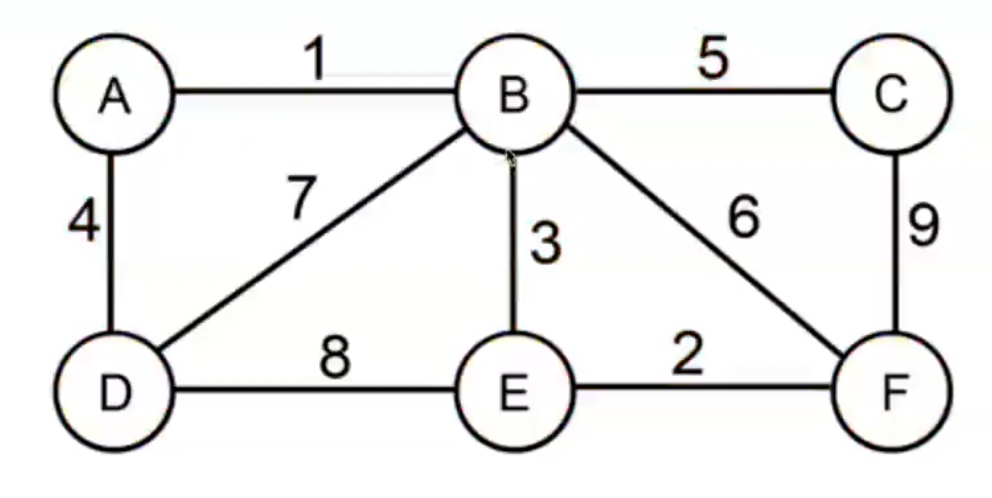
\includegraphics[width=0.4\textwidth]{asset/07406ba2-1bde-448c-a84b-eaf3716aaeb0.jpg}
  \caption{}
  \label{fig:img27_6}
\end{figure}

先来看一下这里有 6 个顶点, 这些边的权重也都告诉我们了. 所以这些边的权重就是从 1-9. 我们按照刚才那个算法的思想, 首先从权重最小这个边开始. 

本来在图里面, a、b、c、d、e、f 这六个点都是孤立的, 它们都是没有边相连的. 然后我们是按照这些边权重从小到大的顺序一个一个去看. 我们就直到这 6 个点全部都被包含了, 形成了一个生成树为止. 

比如说第一条, 边权重最小 1(图: \ref{fig:img27_7}, \ref{fig:img27_8}):

\begin{figure}[ht]
  \centering
  \begin{minipage}[t]{0.4\textwidth}
    \centering
    \caption{}
    \label{fig:img27_7}
    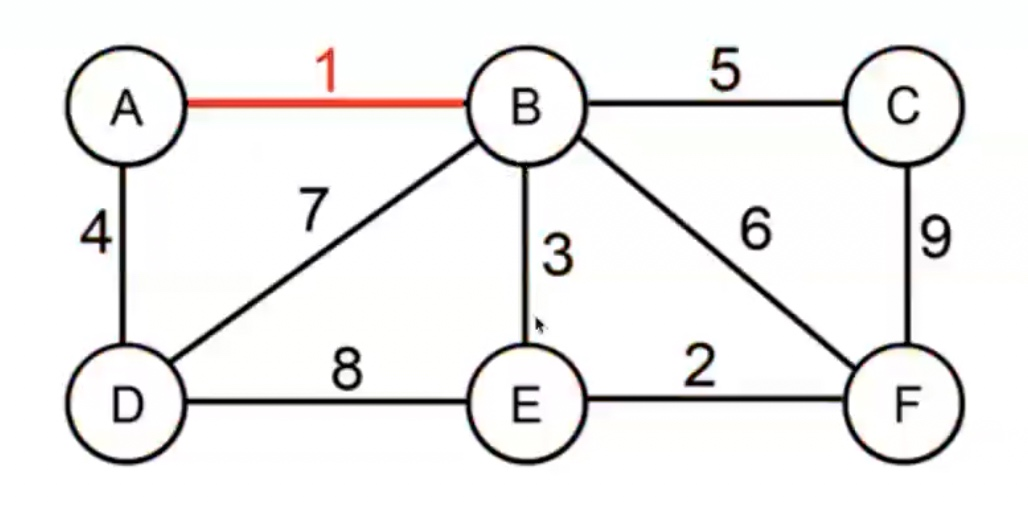
\includegraphics[width=\textwidth]{asset/aefaaf0e-21e1-4505-aff2-907f9932b2b3.jpg}
  \end{minipage}%
  \hspace{1em}
  \begin{minipage}[t]{0.4\textwidth}
    \centering
    \caption{}
    \label{fig:img27_8}
    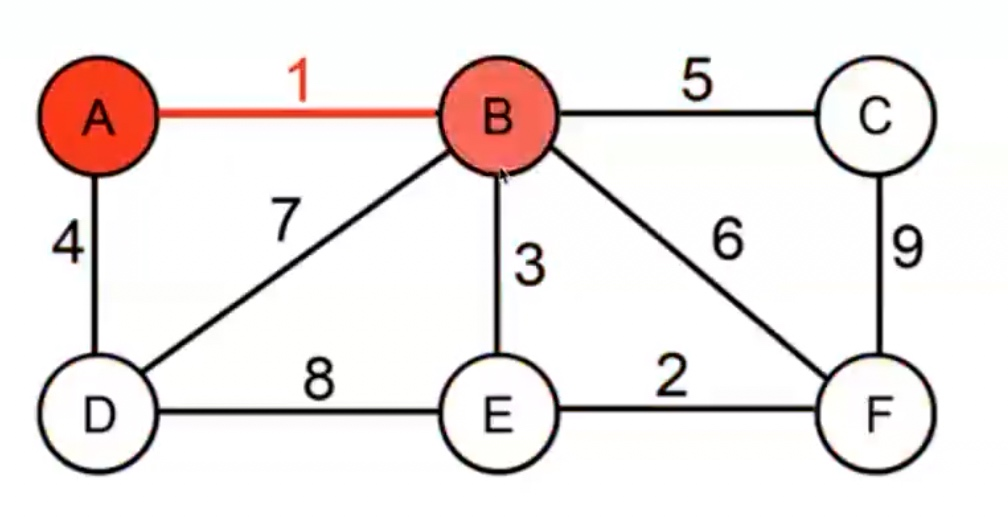
\includegraphics[width=\textwidth]{asset/9d0be540-499d-4d9b-9b9b-d3ed959381cf.jpg}
  \end{minipage}
\end{figure}

接下来就是 2, EF 也是属于不同树(图: \ref{fig:img27_9}, \ref{fig:img27_10}): 

\begin{figure}[ht]
  \centering
  \begin{minipage}[t]{0.4\textwidth}
    \centering
    \caption{}
    \label{fig:img27_9}
    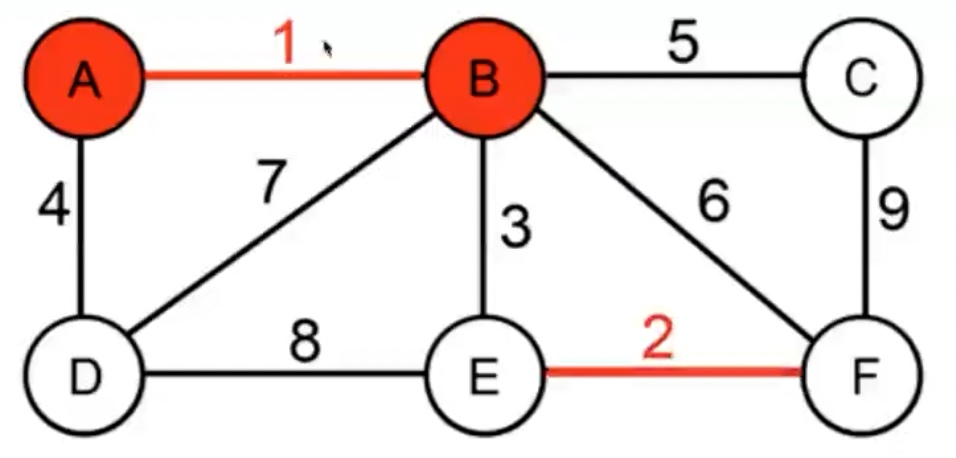
\includegraphics[width=\textwidth]{asset/2c867981-cf42-4372-b2de-0b95d4f1729a.jpg}
  \end{minipage}%
  \hspace{1em}
  \begin{minipage}[t]{0.4\textwidth}
    \centering
    \caption{}
    \label{fig:img27_10}
    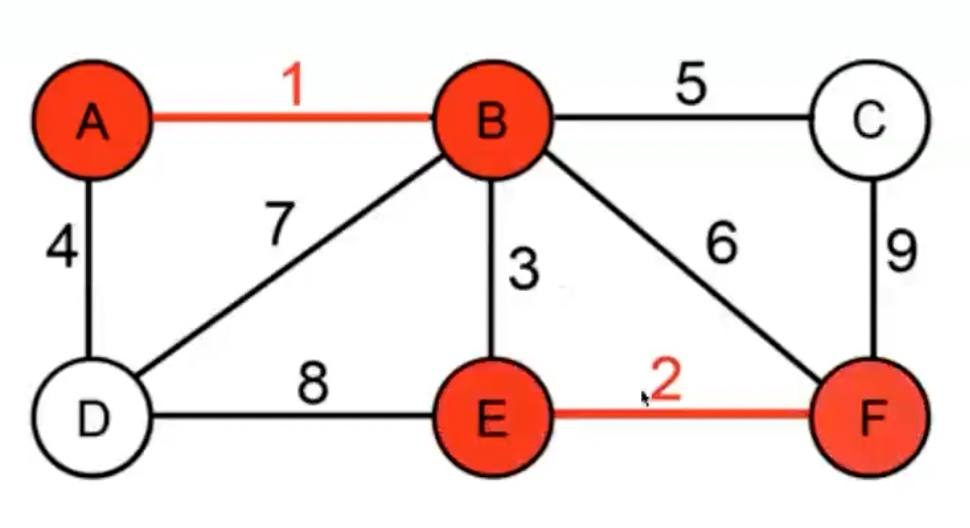
\includegraphics[width=\textwidth]{asset/c2333fd2-d4a4-4d44-8381-9d0dd9588789.jpg}
  \end{minipage}
\end{figure}

接下来选中 3, 大家注意一下在 3 之前, 这里已经 AB 连上了、EF 连上了, 那这时候 3 连上了代表什么?AB 这个时候是一棵树, EF 是一颗数, 这时候 BE 分别属于两个树, 符合规则定义, 所以 3 可以选. (图: \ref{fig:img27_11})

\begin{figure}[ht]
  \centering
  \caption{}
  \label{fig:img27_11}
  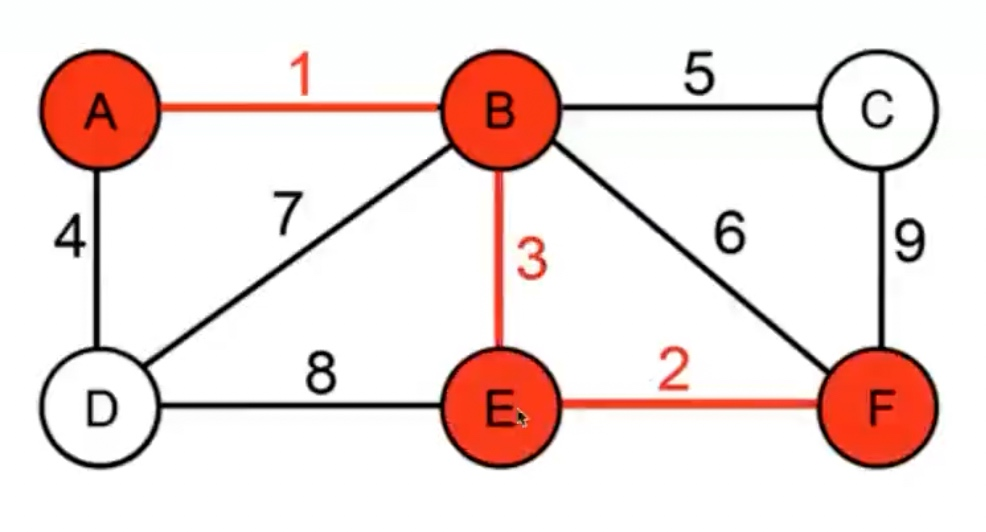
\includegraphics[width=0.4\textwidth]{asset/c24feadf-69a2-46d0-af7e-dae86d8956ab.jpg}
\end{figure}

接下来按照递增的顺序, 123 都选择之后, 最小的就是 4 了, 4 它也 OK. A 属于 ABE 这条树, D 是一个孤立的点, 所以把 4 给勾上 (图: \ref{fig:img27_12}, \ref{fig:img27_13}). 

\begin{figure}[ht]
  \centering
  \begin{minipage}[t]{0.4\textwidth}
    \centering
    \caption{}
    \label{fig:img27_12}
    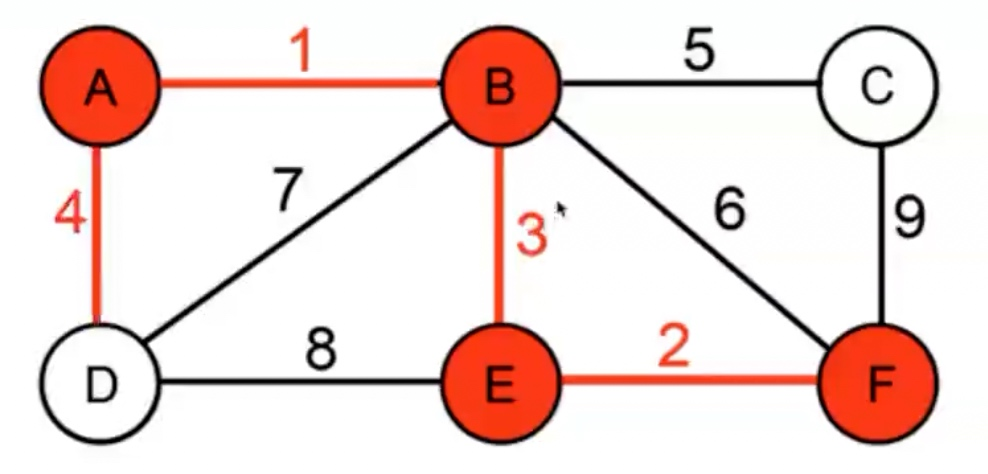
\includegraphics[width=\textwidth]{asset/90cfb2e1-d182-4637-a969-08136f9db0f3.jpg}
  \end{minipage}%
  \hspace{1em}
  \begin{minipage}[t]{0.4\textwidth}
    \centering
    \caption{}
    \label{fig:img27_13}
    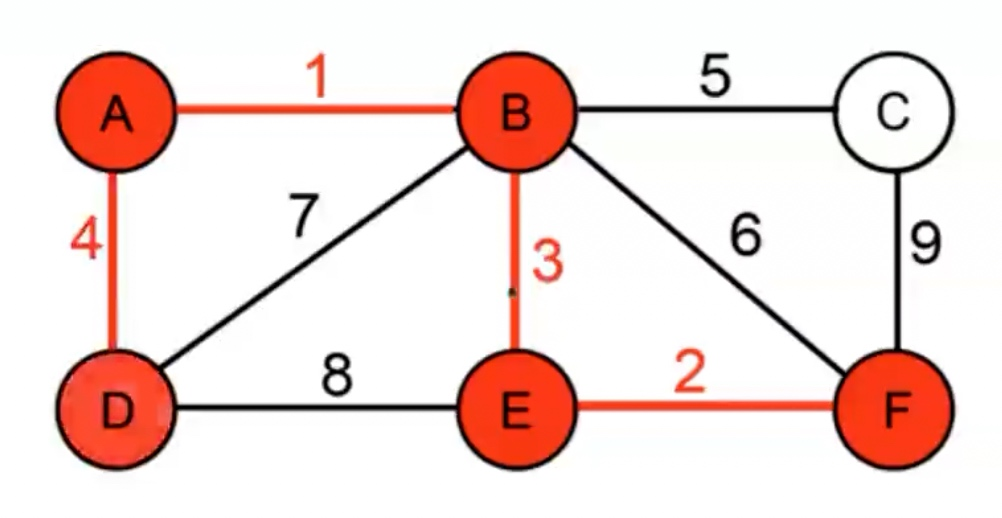
\includegraphics[width=\textwidth]{asset/0d6a03e3-624d-4dfc-a8b8-ee7bc651cf5a.jpg}
  \end{minipage}
\end{figure}

它也就是把两个属于不同树的顶点给它结合在一起了. 

最后一步到 5, 道理也是一样, 到 5 这一步为止了(图: \ref{fig:img27_14}, \ref{fig:img27_15}): 

\begin{figure}[ht]
  \centering
  \begin{minipage}[t]{0.4\textwidth}
    \centering
    \caption{}
    \label{fig:img27_14}
    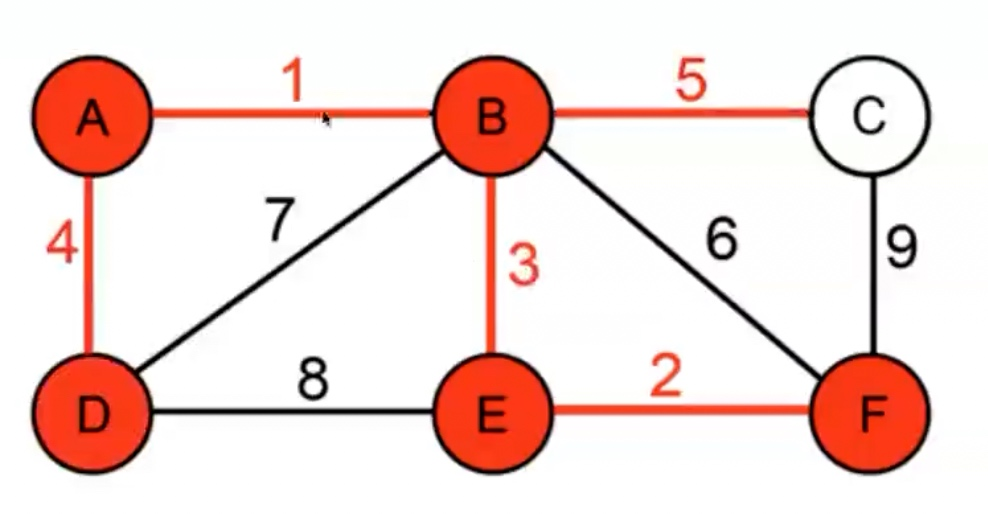
\includegraphics[width=\textwidth]{asset/01a127e3-24ba-4f89-8ce7-fe6fce090e4f.jpg}
  \end{minipage}%
  \hspace{1em}
  \begin{minipage}[t]{0.4\textwidth}
    \centering
    \caption{}
    \label{fig:img27_15}
    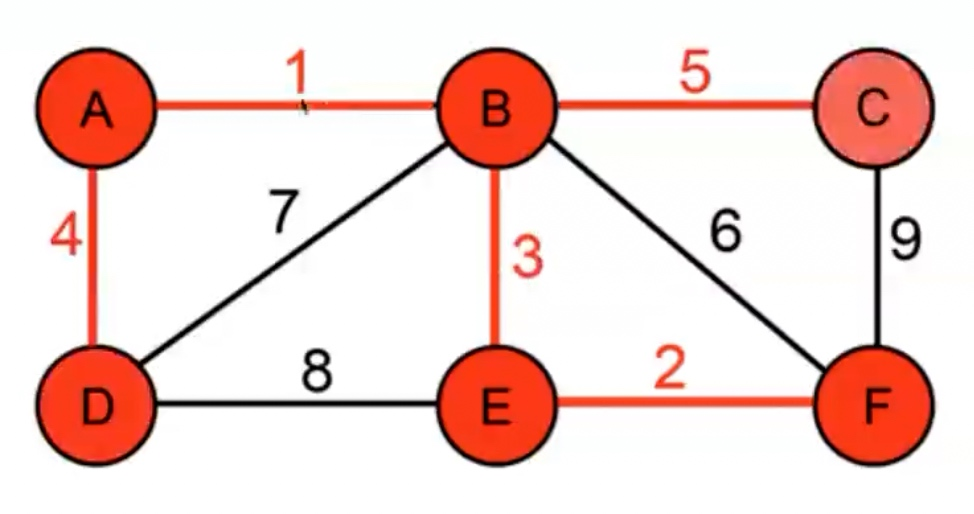
\includegraphics[width=\textwidth]{asset/9fef2b67-86cd-49ba-812d-a3e920ee59f3.jpg}
  \end{minipage}
\end{figure}

我们会发现这 6 点已经都被囊括在内了, 所以我们就停手了. 这样最小生成树也就形成了. 

好, 问题来了. 在这种情况下, 为什么就能说它产生的这个生成树就是最小权重生成树?大家可以想一下为什么. 

其实道理非常非常简单. 因为我们挑选权重, 挑选的这个边是按照从小到大的顺序对权重去进行一个排序, 就是我们想尽可能的用这个最小权重的边去构成这个生成树. 所以按照从小到大顺序去进行排列挑出来这些边, 他一定是符合这个原则的. 按照这种算法得到的生成树一定是最小生成树. 

这个例子刚好按照 12345 的这个顺序, 所有边都可以. 那如果说它是有一些特例的情况, 比如说 AB, 然后 EF, AB、EF 已经连上了之后 BF 之间是 4, 那这个时候我们这 BF 就不能选了, 因为在选 BF 之前, ABEF 已经在共同的一棵树上面了. 这时候选 BF 这条边, BF 对应的两个点是在一条树上面, 所以是不符合第四步的, BF 这条边就不能选. 

什么意思呢?就是说, 虽然 BF 长度权重是 4, AD 是 6, 但我们第四步会看到 BF 这个边. 这种情况 BF 是不能选, 因为它 ABEF 是在一条树上面. 

只不过是我们所讲解的这个动图里面是按照 12345 的这个顺序, 刚好可以构成一个最小生成树. 

那如果是一些权重是相同怎么办?权重相同的话, 就随便选一个都行. 权重相同的话就无所谓了, 选哪一个都 OK, 没有任何影响. 

\section{图与人工智能}

好, 接下来我们要讲的, 是我们这节课最后一个内容. 这部分内容不涉及到任何关于数学方面的东西了, 就是给大家说一下图论和这个人工智能会有哪些相交叉的部分. 

相对而言, 图虽然近些年来有图神经网络, 是针对图的结构去做的一种优化, 去做智能方面的一些处理, 但是相对于其他数学领域, 图用的频率还不是特别的多. 但是它的用途其实比较广泛了. 

比如, 社交网络的一个分析. 你在 Facebook 上面和你的朋友, Facebook 就会认为你们既然是朋友, 那你们肯定会有一些共通的兴趣爱好. 所以有一天你的朋友如果点了了一个 like, 或者说点赞了某一个话题, 或者说进了某一个 topic. 你朋友这样做的话, Facebook 系统可能也会给你去推送这么样一个邀请. 

比如邀请你加入这个话题小组, 邀请你去探讨一下这个领域的一个话题. 或者说, 你有两个朋友, 你是 a, 你有两个朋友 b 和 c, 然后 b 和 c 都认识 d, 那这个时候 Facebook 或者说领英这样的社交平台可能就会给你推荐好友. 既然 b 和 c 都认识 d, 那你认识 d 的可能性也比较大, 谁让你们 3 个是朋友呢. 所以他就会给你推荐朋友, 把 d 给到你. 

这个也是根据一个相似性来去做的一个判断, 也是用到这种图的一个结构. 

然后我们还有一个应用, 电商平台的这种商品推荐. 想必大家对这个印象可能会更深一点. 因为我们在国内的这种购物平台, 京东、淘宝、天猫啊这些去买书, 你选了一个历史类的, 比如你买了一本北周到唐代的府兵制度的一个考试, 一个考古文集. 系统可能就会认为你对这种军事制度相关的、历史制度相关的东西很感兴趣, 他之后就会给你推荐这方面的一些书. 可能会给你推荐一些中国兵制, 中国兵器史稿之类的书. 

那再比如你是喜欢看一些法律, 美国的这种三权分立体系, 罗斯福总统在经济大萧条时期怎么样对抗联邦最高法院. 那如果你买了这种书系统也会给你推荐相关的这种法律方面的书. 

所以说, 我们在这里也会用到图的这么一个结构, 也是基于这种相似度, 基于图的这种结构. 

剩下这两个例子比较类似的, 一个是车辆的、一个路径规划, 我从 AD 要到 BD, 这个最短路径怎么样去求出来?有的可能是用 Dijkstra 算法, 但是 Dijkstra 算法只考虑了距离, 我们在实际运用当中可能还要考虑到红绿灯怎么样. 

或者说如果你想省钱的话, 这条路虽然快虽然近, 但是是一个高速路. 要花钱, 你不愿意, 那怎么办呢?那所以他就会给你一些路径偏好的设置, 会给你一些选择. 

你是要快速, 还是要躲避拥堵, 还是要少红绿灯呢. 大家用过高德、百度导航, 都有过这样的经历. 

然后港口的叉车调度什么的其实也是一样. 就是一个码头一个港口, 或者说一个物流仓储的一个仓库. 你这些机器人, 比如有多个包裹要放在多个货架上面, 不同的货架上面怎么样安排这个路径, 使得机器人走的总路径是最小的, 你怎么样去算. 

\begin{figure}[ht]
  \centering
  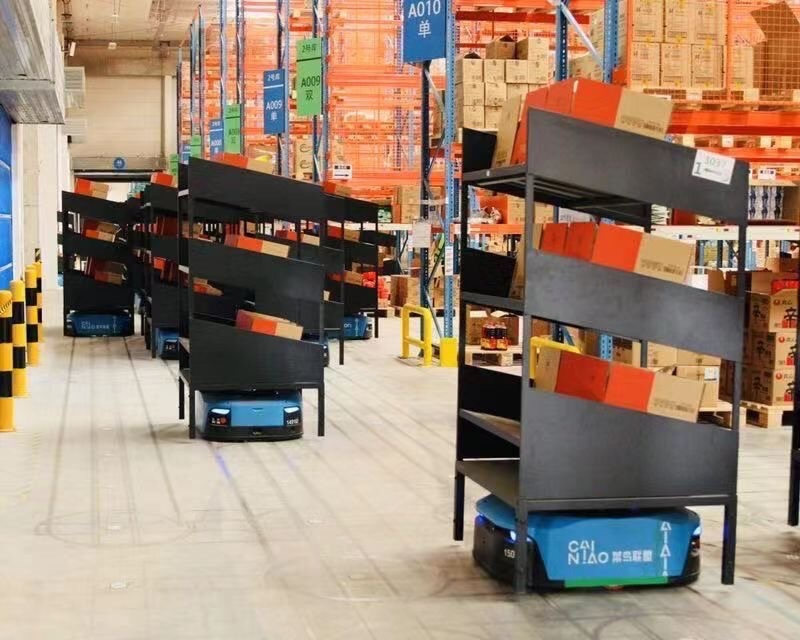
\includegraphics[width=0.5\textwidth]{asset/aca75bfd-73da-4714-98d3-2f60e8401afd.jpg}
\end{figure}

\begin{figure}[ht]
  \centering
  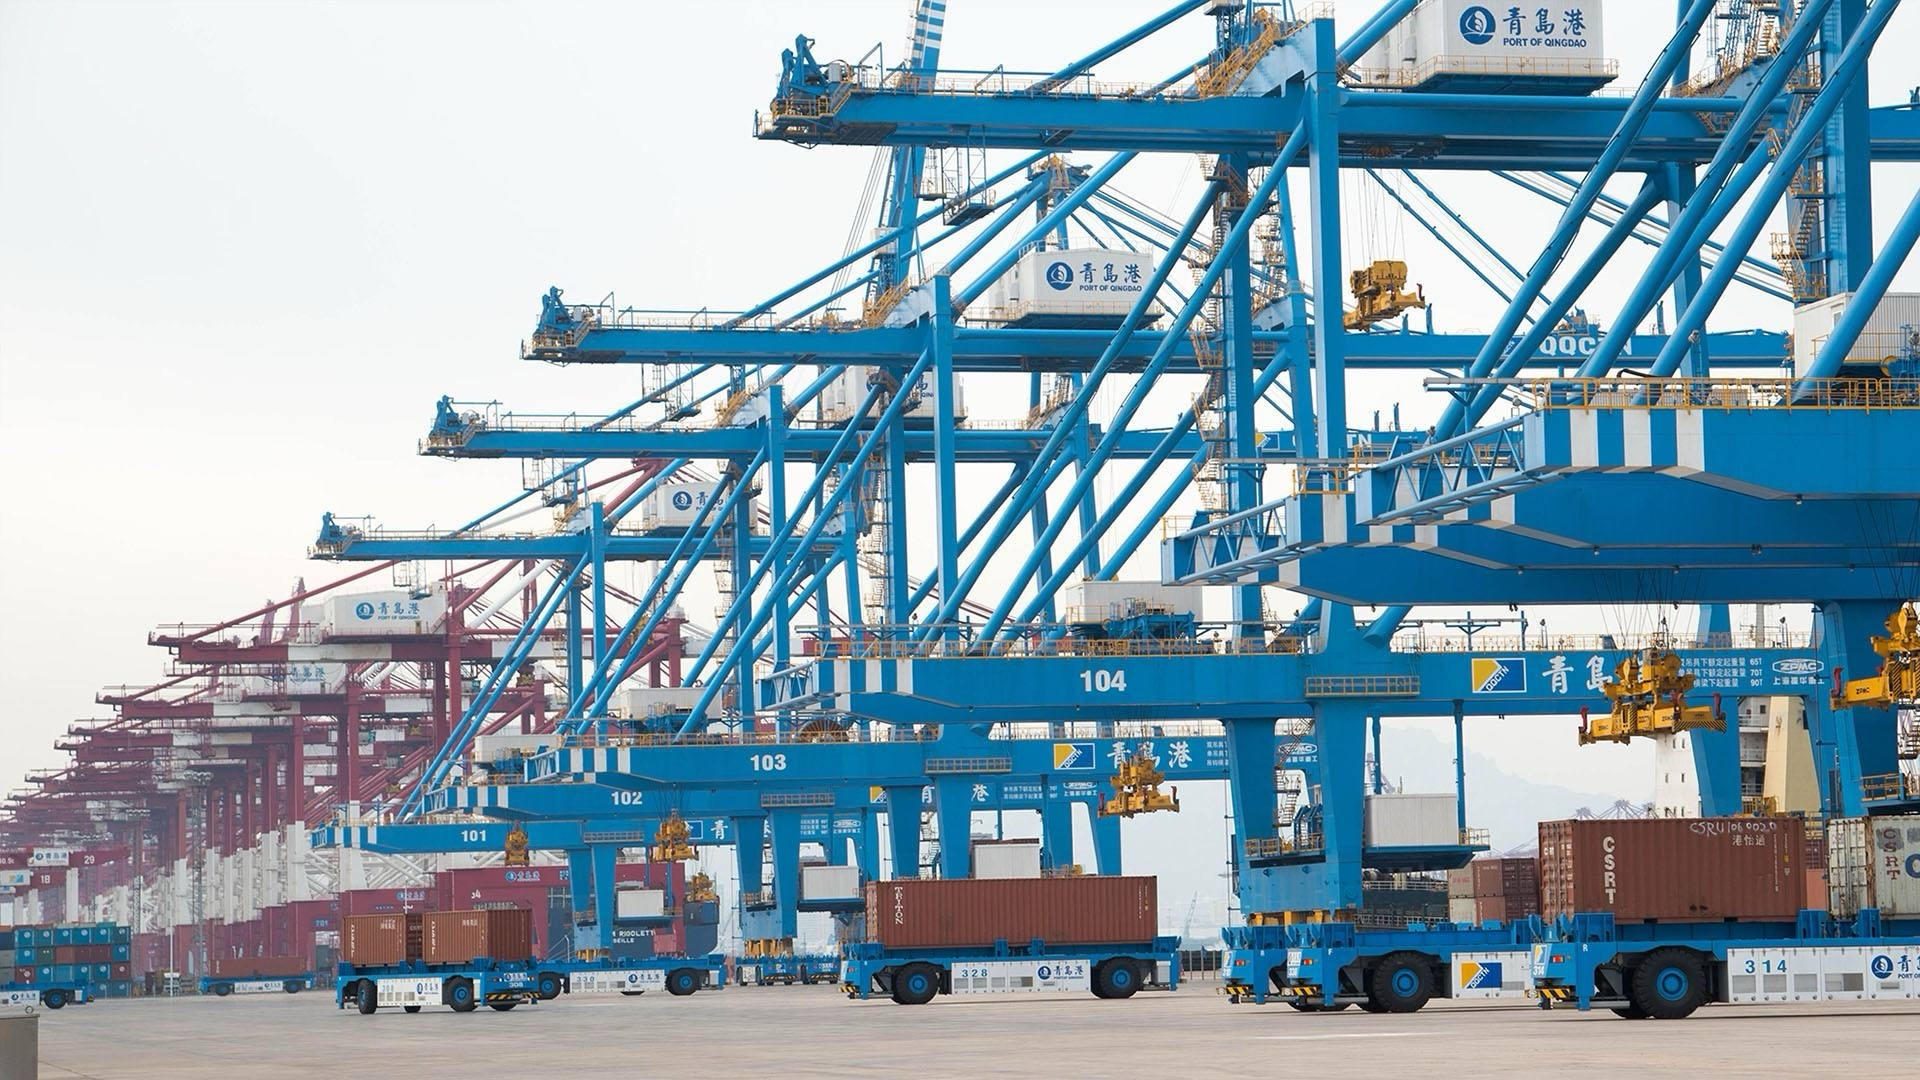
\includegraphics[width=0.5\textwidth]{asset/3327fbab-a005-4963-a7e9-b413f9ac1c84.jpg}
\end{figure}

这部分也也是和图有关的, 也是基于图的这种结构. 就类似于我们讲解 Dijkstra 算法这种思想. 

\section{人工智能数学基础}

那最后, 我们也就是来到了这节课的末尾了. 我相信大家通过这 26 节课的学习, 或多或少的会对人工智能里面所涉及到的一些数学方面的内容有了一些基本性的了解. 当然了, 我在这里呢也给大家一些建议, 也是我个人觉得, 大家如果是没有进入这个行业的话, 没有进入人工智能这个领域的话, 你怎么样处理和数学相关的这个知识的一些建议. 

第一点, 不用翻字典. 这个我说过很多次了, 大家也看过很多次. 

给你一本技术手册, 或者说给你一个 document, 是关于这个 Python 语法的, 或者说整本的关于高等代数的. 我是不推荐你们在学习人工智能的时候去一页不差的去看那些书. 

我们怎么样去学呢?你主要是看人工智能相关的书, 如果你在人工智能里面的这些书籍看到和数学相关, 但是你不懂东西, 再去查那些数学书, 或者去 Google. 把你的问题抛出来, Google 能出来很多结果, 不要自己去一页一页的翻这些 document, 去翻这些字典性的技术性手册. 

我可以告诉你这个没有任何用, 因为不是所有人都是俞敏洪, 不是所有人都是靠背字典学会英语的. 也不是通过你背技术手册就能精通一门语言, 或者精通某一个领域. 这些技术性手册更多的是给你在不知道的时候去翻查的. 

最好的方式还是碰到问题你去 Google, 直接把这个答案搜一下. 你在网上看这些解答的过程当中又发现了一些新的问题, 那你就再去查这个知识点, 一环套一环一环. 只有这样子你所学的东西才是必要的, 才能记得非常牢固. 

第二点、循序渐进步步为营. 

这话听起来比较空泛, 但是这话其实我是想表达一个怎么样的意思呢. 就是大家首先不要着急, 因为大家可能有的人会去了解一下一些很复杂的神经网络的结构, 那种超大规模神经网络, 那你可能就会觉得: 我的天, 我怎么可能从零开始搭建出这么复杂的一个网络. 

其实我是这样觉得的, 就是这个跟我们导论课里面说的一样. 我说过, 不管你多么复杂的电路它最基本的就是那三种门电路. 我不知道大家还有多少人记得, 如果不记得再回去看一下. 

就是不管晶片里面是包含了几千亿个或者说几十亿个电路单元, 它最基本的组成单位都是那三个. 通过这三个的组合, 你才形成了千种万种的复杂的结构. 

所以我们学人工智能也是一样, 什么东西呢都是一点一点累出来的. 

你先学会神经网络是包含了哪些结构, 对于这种图像, 可能卷积神经网络用的比较多一点, 那它会有一个特殊的卷积层. 然后它还有一个池化层, 它是干什么的. 

然后在这个计算机视觉领域里面, 它主要都是靠这些层来堆积起来的. 可能堆积的方式不同, 这里面会有些小技巧, 但是它的骨架都是一样的. 

希望大家就是说在我的课里面能一切顺利, 学有所成, 学到自己想要的知识. 对于想转行, 想转进 AI 这个领域的同学, 祝愿你们能成功如愿, 拿到一份更高薪的工作. 

对于目前还在学校的同学, 也希望你们毕业了之后进入社会后第一份工作就能非常好. 

这个数学课有什么不太明白的地方, 自己再多回看理解一下, 或者去找其他资料对应着来学习. 顺便培养下自己主动解决问题的一个能力. 

因为最终只有你自己能帮你自己解决问题, 老师都只是在一节路上去带你. 

好, 那我们的《茶桁 AI 秘籍 - 数学篇》也就随着本节课结束全部结束了. 大家可以等一段时间, 然后跟随我一起进入真正的 AI 大门. 

按照规划, 咱们下一节课开始进入真正的《AI 核心基础能力》

咱们会从「人工智能导论」开始, 详细的介绍机器学习, 然后是 RNN、CNN, 再之后我们会讲解一些自然语言处理, 计算机视觉以及商业智能的相关基础. 

OK, 咱们所有课程到这里就结束了, 最后祝大家一切顺利. 

